\title[Resonant converters II]{Resonant converters II: VHF inverters, rectifiers and matching networks}
\section{Resonant converters II}

\begin{frame}[plain]
	\titlepage
\end{frame}

%%%%%%%%%%%%%%%%%%%%%%%%%%%%%%%%%%%%%%%%%%%%%%%%%%%%%%%%%%%%%
%% Overview %%
%%%%%%%%%%%%%%%%%%%%%%%%%%%%%%%%%%%%%%%%%%%%%%%%%%%%%%%%%%%%%
\subsection{Single-switch topologies}

\begin{frame}
	\frametitle{Overview}
	L9 used a half-bridge and a tank up to about 1\,MHz. Above 10\,MHz the switch itself becomes the problem: its capacitance, its drive and its timing.
	\begin{itemize}
		\item Why one switch: ground-referenced drive, $C_\mathrm{oss}$ inside the tank
		\item Class E: design equations, frequency limit, load sensitivity
		\item Class $\Phi_2$ and class DE
		\item Resonant rectifiers, resistance compression and matching networks
		\item The VHF dc--dc converter with on/off control
		\item Wireless power and industrial RF; components, layout and measurement
	\end{itemize}
	After this lecture you can design a class E inverter and an L-section matching network for 6.78 to 30\,MHz and judge whether a transistor is small enough for the frequency.
\end{frame}

%%%%%%%%%%%%%%%%%%%%%%%%%%%%%%%%%%%%%%%%%%%%%%%%%%%%%%%%%%%%%
%% Why one switch %%
%%%%%%%%%%%%%%%%%%%%%%%%%%%%%%%%%%%%%%%%%%%%%%%%%%%%%%%%%%%%%
\begin{frame}
	\frametitle{Why one switch above 10\,MHz}
	\begin{columns}[T]
		\begin{column}{0.48\textwidth}
			\footnotesize
			\textbf{Half-bridge at 13.56\,MHz}
			\begin{itemize}
				\item The period is 73.7\,ns. A ZVS transition takes $2Q_\mathrm{oss}/I$: 5\,ns for $Q_\mathrm{oss}=5$\,nC and $I=2$\,A (L8), already 14\,\% of the half period.
				\item The high-side switch needs a level shifter or an isolated supply; its delay and the spread of this delay must stay small against the dead time (L4).
				\item Two gate drives, each dissipating $Q_\mathrm{G}V_\mathrm{GS}f$: 0.47\,W per switch for the 100\,V GaN transistor of L4 (7\,nC at 5\,V).
			\end{itemize}
		\end{column}
		\begin{column}{0.48\textwidth}
			\footnotesize
			\textbf{Single switch}
			\begin{itemize}
				\item Source at ground: a simple gate driver.
				\item $C_\mathrm{oss}$ and stray capacitance are part of the tank.
				\item The switch turns on at zero voltage and zero $\mathrm{d}v/\mathrm{d}t$: slow gate edges and small timing errors cost little.
				\item A resonant driver can recover the gate energy (L4).
				\item The price: a switch voltage of 2.4 to 3.6 times the input voltage, and tuning for one operating point.
			\end{itemize}
		\end{column}
	\end{columns}
	\begin{block}{Key message}
		Above 10\,MHz the circuit is built around the switch and its capacitance.
	\end{block}
	\blfootnote{Sources: Sokal and Sokal, 1975; D.\,J. Perreault et al., IEEE APEC 2009.}
\end{frame}

%%%%%%%%%%%%%%%%%%%%%%%%%%%%%%%%%%%%%%%%%%%%%%%%%%%%%%%%%%%%%
%% What changes at VHF %%
%%%%%%%%%%%%%%%%%%%%%%%%%%%%%%%%%%%%%%%%%%%%%%%%%%%%%%%%%%%%%
\begin{frame}
	\frametitle{What changes at VHF}
	\begin{columns}[T]
		\begin{column}{0.44\textwidth}
			\begin{table}
				\centering
				\footnotesize
				\begin{tabular}{|l|c|c|}
					\hline
					                                         & Si LDMOS     & GaN HEMT     \\
					                                         & MRF6S9060    & CGH40045     \\
					\hline
					$R_\mathrm{DS}$                          & 175\,m$\Omega$ & 200\,m$\Omega$ \\
					$C_\mathrm{oss}$                         & 50\,pF       & 8.3\,pF      \\
					$V_\mathrm{br}$                          & 68\,V        & 100\,V       \\
					$R_\mathrm{DS}C_\mathrm{oss}$            & 8.8\,ps      & 1.7\,ps      \\
					\hline
				\end{tabular}
				\caption{Two RF transistors: on-resistance $R_\mathrm{DS}$, output capacitance $C_\mathrm{oss}$, breakdown voltage $V_\mathrm{br}$; a smaller $R_\mathrm{DS}C_\mathrm{oss}$ is better (Perreault et al., 2009)}
			\end{table}
		\end{column}
		\begin{column}{0.53\textwidth}
			\footnotesize
			\begin{itemize}
				\item Switches: a smaller device has less $C_\mathrm{oss}$ but more $R_\mathrm{DS}$; the product $R_\mathrm{DS}C_\mathrm{oss}$ limits the frequency. ZVS removes the $C_\mathrm{oss}V^2f$ loss, but the current that charges $C_\mathrm{oss}$ still flows.
				\item Magnetics: ferrite core loss limits the flux density; above about 10\,MHz air-core inductors or low-$\mu$ RF materials are used (L6, L7).
				\item Interconnect: a few nH of loop inductance are a noticeable part of each tank reactance (1\,nH is 0.19\,$\Omega$ at 30\,MHz) and must be absorbed into the tank.
				\item Control: PWM within a period of 74\,ns (13.56\,MHz) is impractical; the whole converter is switched on and off instead (later in this lecture).
			\end{itemize}
		\end{column}
	\end{columns}
	\blfootnote{Source: D.\,J. Perreault et al., ``Opportunities and challenges in very high frequency power conversion,'' IEEE APEC 2009, Table II.}
\end{frame}

%%%%%%%%%%%%%%%%%%%%%%%%%%%%%%%%%%%%%%%%%%%%%%%%%%%%%%%%%%%%%
%% Class E inverter %%
%%%%%%%%%%%%%%%%%%%%%%%%%%%%%%%%%%%%%%%%%%%%%%%%%%%%%%%%%%%%%
\subsection{Class E inverter}

\begin{frame}
	\frametitle{The class E inverter}
	\begin{columns}[T]
		\begin{column}{0.52\textwidth}
			\begin{figure}
				\centering
				\begin{circuitikz}[scale=0.78, transform shape]
					\draw (0,0) to[V, l=$V_\mathrm{DC}$] (0,3.2) to[L, l=$L_\mathrm{F}$, i>^=$I_\mathrm{DC}$] (2.6,3.2) node[circ]{};
					\draw (2.6,3.2) -- (2.6,2.5) node[nigfete, anchor=D] (S) {};
					\draw (S.S) -- (2.6,0) node[circ]{};
					\node[anchor=east] at (S.G) {S};
					\draw (2.6,3.2) -- (4.0,3.2) to[C, l=$C_\mathrm{sh}$, v_>=$v_\mathrm{S}$] (4.0,0) node[circ]{};
					\draw (4.0,3.2) to[L, l=$L$, i>^=$i_\mathrm{o}$] (6.0,3.2) to[C, l=$C_0$] (7.6,3.2) to[R, l=$R$] (7.6,0) -- (0,0);
				\end{circuitikz}
				\caption{Class E inverter. At the switching frequency the series branch $L$--$C_0$ is inductive by the excess reactance $X=\omega L-1/(\omega C_0)>0$}
			\end{figure}
		\end{column}
		\begin{column}{0.46\textwidth}
			\footnotesize
			\begin{itemize}
				\item S is on for half the period ($D=0.5$). At turn-off, $C_\mathrm{sh}$ (including $C_\mathrm{oss}$) takes over the current and holds $v_\mathrm{S}$ low while the channel current falls.
				\item The choke $L_\mathrm{F}$ carries a nearly constant $I_\mathrm{DC}$; the branch $L$--$C_0$ passes a nearly sinusoidal $i_\mathrm{o}$ to $R$.
				\item $X$ sets the phase of $i_\mathrm{o}$ and thus the shape of $v_\mathrm{S}$ while S is off. It is chosen for zero voltage (ZVS) and zero slope (ZDS, zero derivative) at turn-on:
				\begin{equation*}
					v_\mathrm{S}=0,\qquad \frac{\mathrm{d}v_\mathrm{S}}{\mathrm{d}t}=0
				\end{equation*}
				\item A turn-on slightly early or late then still finds $v_\mathrm{S}\approx0$: timing errors cost almost nothing.
			\end{itemize}
		\end{column}
	\end{columns}
	\blfootnote{Sources: Sokal and Sokal, IEEE JSSC, 1975 (96\,\% transistor efficiency at 3.9\,MHz, 26\,W); Raab, IEEE Trans.\ Circuits Syst., 1977.}
\end{frame}

%%%%%%%%%%%%%%%%%%%%%%%%%%%%%%%%%%%%%%%%%%%%%%%%%%%%%%%%%%%%%
%% Class E waveforms %%
%%%%%%%%%%%%%%%%%%%%%%%%%%%%%%%%%%%%%%%%%%%%%%%%%%%%%%%%%%%%%
\begin{frame}
	\frametitle{Class E waveforms}
	\begin{columns}[T]
		\begin{column}{0.52\textwidth}
			\begin{figure}
				\centering
				\begin{tikzpicture}
					\begin{groupplot}[
							group style={group size=1 by 2, vertical sep=0.25cm, xticklabels at=edge bottom},
							width=\linewidth, height=3.2cm,
							xmin=0, xmax=360, xtick={0,90,180,270,360},
							grid=major, grid style={gray!20},
							tick label style={font=\scriptsize}, label style={font=\footnotesize},
						]
						\nextgroupplot[ymin=-0.3, ymax=4, ytick={0,1,2,3,4}, ylabel={$v_\mathrm{S}/V_\mathrm{DC}$}]
						\addplot[black, thick] table[x=th, y=v] {fig/lec10/classe_ideal.dat};
						\node[font=\tiny, anchor=south] at (axis cs:90,0.05) {switch on};
						\node[font=\tiny, anchor=south] at (axis cs:300,3.25) {switch off};
						\nextgroupplot[ymin=-2.2, ymax=3.3, ytick={-2,-1,0,1,2,3}, ylabel={$i/I_\mathrm{DC}$}, xlabel={$\theta=\omega t$ ($^\circ$)}]
						\addplot[black, thick] table[x=th, y=i] {fig/lec10/classe_ideal.dat};
						\addplot[black, dashed] table[x=th, y=io] {fig/lec10/classe_ideal.dat};
						\node[font=\tiny, anchor=south] at (axis cs:60,2.0) {$i_\mathrm{S}$};
						\node[font=\tiny, anchor=south] at (axis cs:300,1.9) {$i_\mathrm{o}$};
					\end{groupplot}
				\end{tikzpicture}
				\caption{Ideal class E ($D=0.5$, $Q_\mathrm{L}\to\infty$). Top: switch voltage; bottom: switch current $i_\mathrm{S}$ (solid) and output current $i_\mathrm{o}$ (dashed)}
			\end{figure}
		\end{column}
		\begin{column}{0.46\textwidth}
			\small
			\begin{itemize}
				\item On ($0$ to $180^\circ$): $i_\mathrm{S}=I_\mathrm{DC}-i_\mathrm{o}$ starts at zero, peaks at $2.86\,I_\mathrm{DC}$ and is $2\,I_\mathrm{DC}$ at turn-off.
				\item Off: $C_\mathrm{sh}$ takes $I_\mathrm{DC}-i_\mathrm{o}$; $v_\mathrm{S}$ peaks at $3.56\,V_\mathrm{DC}$ at $245^\circ$ and returns to zero with zero slope.
				\item The two conditions ZVS and ZDS fix amplitude and phase of the output current: $i_\mathrm{o}=1.86\,I_\mathrm{DC}\sin(\theta+147.5^\circ)$.
				\item The remaining switching loss is the turn-off at $2\,I_\mathrm{DC}$: the channel must open before $C_\mathrm{sh}$ has charged noticeably (L8).
			\end{itemize}
		\end{column}
	\end{columns}
	\blfootnote{Analytical solution after Raab, 1977 (\texttt{lecture/sim/classe\_timedomain.py}).}
\end{frame}

%%%%%%%%%%%%%%%%%%%%%%%%%%%%%%%%%%%%%%%%%%%%%%%%%%%%%%%%%%%%%
%% Design equations %%
%%%%%%%%%%%%%%%%%%%%%%%%%%%%%%%%%%%%%%%%%%%%%%%%%%%%%%%%%%%%%
\begin{frame}
	\frametitle{Design equations}
	\begin{columns}[T]
		\begin{column}{0.5\textwidth}
			\footnotesize
			Assumptions: $D=0.5$, $Q_\mathrm{L}\to\infty$ (sinusoidal $i_\mathrm{o}$), $L_\mathrm{F}\to\infty$, linear $C_\mathrm{sh}$, ideal switch.
			\begin{itemize}
				\item Off interval ($\pi<\theta<2\pi$): $C_\mathrm{sh}$ carries $I_\mathrm{DC}-i_\mathrm{o}$, with $i_\mathrm{o}=I_\mathrm{m}\sin(\theta+\varphi)$:
				\begin{equation*}
					\omega C_\mathrm{sh}\,\frac{\mathrm{d}v_\mathrm{S}}{\mathrm{d}\theta}=I_\mathrm{DC}-I_\mathrm{m}\sin(\theta+\varphi)
				\end{equation*}
				\item Integrate and require $v_\mathrm{S}=0$ and $\mathrm{d}v_\mathrm{S}/\mathrm{d}\theta=0$ at $\theta=2\pi$:
				\begin{equation*}
					I_\mathrm{m}\sin\varphi=I_\mathrm{DC},\qquad I_\mathrm{m}\cos\varphi=-\frac{\pi}{2}I_\mathrm{DC}
				\end{equation*}
				\item The mean of $v_\mathrm{S}$ equals $V_\mathrm{DC}$ ($L_\mathrm{F}$ has no DC voltage). The fundamental of $v_\mathrm{S}$ in phase with $i_\mathrm{o}$ drops across $R$, the part in quadrature across $X$: this gives $R$ and $X$.
			\end{itemize}
		\end{column}
		\begin{column}{0.47\textwidth}
			\begin{varblock}[\textwidth]{Class E, $D=0.5$, $Q_\mathrm{L}\to\infty$}
				\footnotesize
				\begin{align*}
					R                       & =\frac{8}{\pi^2+4}\,\frac{V_\mathrm{DC}^2}{P}=0.5768\,\frac{V_\mathrm{DC}^2}{P} \\
					\omega C_\mathrm{sh}R   & =\frac{8}{\pi(\pi^2+4)}=0.1836                                                 \\
					X                       & =\frac{\pi(\pi^2-4)}{16}\,R=1.1525\,R                                          \\
					V_\mathrm{S,pk}         & =3.562\,V_\mathrm{DC},\qquad I_\mathrm{S,pk}=2.862\,I_\mathrm{DC}
				\end{align*}
				Output power per switch stress $P/(V_\mathrm{S,pk}I_\mathrm{S,pk})=0.098$ (power-output capability; class D: 0.159, both switches counted).
			\end{varblock}
		\end{column}
	\end{columns}
	\blfootnote{Sources: Raab, 1977; M.\,K. Kazimierczuk, \textit{RF Power Amplifiers}, 2nd ed., Wiley, 2014.}
\end{frame}

%%%%%%%%%%%%%%%%%%%%%%%%%%%%%%%%%%%%%%%%%%%%%%%%%%%%%%%%%%%%%
%% Task: class E for B5 %%
%%%%%%%%%%%%%%%%%%%%%%%%%%%%%%%%%%%%%%%%%%%%%%%%%%%%%%%%%%%%%
% Two pages: task (page 1) and task with solution (page 2).
\begin{frame}<handout:1-2>
	\frametitle{Class E for brief B5}
	\begin{block}{Task (4 minutes)}
		Class E inverter for 10\,W from 24\,V at 13.56\,MHz, $D=0.5$, ideal design equations.
		\begin{enumerate}
			\item Calculate $R$, $C_\mathrm{sh}$ and the excess reactance $X$.
			\item Peak switch voltage and current? Which voltage rating?
			\item The layout adds 8\,pF at the drain. What remains for $C_\mathrm{oss}$ and an external capacitor?
		\end{enumerate}
	\end{block}
	\onslide<2-|handout:2>{
		\small
		\begin{enumerate}
			\item $R=0.5768\cdot(24\,\mathrm{V})^2/10\,\mathrm{W}=33.2\,\Omega$; $C_\mathrm{sh}=0.1836/(2\pi\cdot13.56\,\mathrm{MHz}\cdot33.2\,\Omega)=64.9$\,pF; $X=1.1525R=38.3\,\Omega$: the series branch is inductive by 38.3\,$\Omega$, i.e.\ 0.45\,$\mu$H more than the inductance that resonates with $C_0$.
			\item $V_\mathrm{S,pk}=3.56\cdot24\,\mathrm{V}=85.5$\,V; $I_\mathrm{DC}=0.42$\,A, $I_\mathrm{S,pk}=1.19$\,A. A 100\,V transistor leaves little margin, since the nonlinear $C_\mathrm{oss}$ and load changes raise the peak: a 150\,V device or a limited load range.
			\item 56.9\,pF for $C_\mathrm{oss}$ (at the operating voltage) and a C0G capacitor. Each picofarad of layout is 1.5\,\% of $C_\mathrm{sh}$.
		\end{enumerate}
	}
\end{frame}

%%%%%%%%%%%%%%%%%%%%%%%%%%%%%%%%%%%%%%%%%%%%%%%%%%%%%%%%%%%%%
%% Finite loaded Q %%
%%%%%%%%%%%%%%%%%%%%%%%%%%%%%%%%%%%%%%%%%%%%%%%%%%%%%%%%%%%%%
\begin{frame}
	\frametitle{Finite loaded Q}
	\begin{columns}[T]
		\begin{column}{0.46\textwidth}
			\begin{table}
				\centering
				\footnotesize
				\begin{tabular}{|c|c|c|c|c|}
					\hline
					$Q_\mathrm{L}$ & $\omega C_\mathrm{sh}R$ & $X/R$ & $RP/V_\mathrm{DC}^2$ & $V_\mathrm{S,pk}/V_\mathrm{DC}$ \\
					\hline
					5              & 0.209                   & 1.29  & 0.517                & 3.62                            \\
					10             & 0.198                   & 1.21  & 0.550                & 3.59                            \\
					20             & 0.191                   & 1.18  & 0.564                & 3.58                            \\
					$\infty$       & 0.184                   & 1.15  & 0.577                & 3.56                            \\
					\hline
				\end{tabular}
				\caption{Normalised design values for ZVS and ZDS from the exact steady state; $Q_\mathrm{L}=\omega L/R$ with the whole series inductance $L$; row $\infty$: ideal equations}
			\end{table}
		\end{column}
		\begin{column}{0.51\textwidth}
			\footnotesize
			\begin{itemize}
				\item At $Q_\mathrm{L}=10$ against the ideal equations: $\omega C_\mathrm{sh}R$ +8\,\%, $X/R$ +5\,\%, $R$ $-5$\,\%. For given $P$ and $V_\mathrm{DC}$, $C_\mathrm{sh}$ is thus 13\,\% larger. Sokal's fitted design equations (2001) agree with the table within 0.5\,\%.
				\item $Q_\mathrm{L}$ is a compromise. The series inductor ($\omega L=Q_\mathrm{L}R$) carries $i_\mathrm{o}$ and loses about $Q_\mathrm{L}/Q_\mathrm{ind}$ of the output power: 5\,\% for $Q_\mathrm{L}=10$ and an inductor quality factor $Q_\mathrm{ind}=200$. A low $Q_\mathrm{L}$ passes more harmonics to the load. Typical: $Q_\mathrm{L}=5$ to 10.
				\item A finite $L_\mathrm{F}$ (a smaller part and a faster start) shifts the values again: verify by simulation.
			\end{itemize}
		\end{column}
	\end{columns}
	\blfootnote{Simulation: \texttt{lecture/sim/classe\_timedomain.py}, ideal switch, $\omega L_\mathrm{F}=10^4R$; N.\,O. Sokal, ``Class-E RF power amplifiers,'' QEX, Jan./Feb.\ 2001.}
\end{frame}

%%%%%%%%%%%%%%%%%%%%%%%%%%%%%%%%%%%%%%%%%%%%%%%%%%%%%%%%%%%%%
%% Maximum frequency %%
%%%%%%%%%%%%%%%%%%%%%%%%%%%%%%%%%%%%%%%%%%%%%%%%%%%%%%%%%%%%%
\begin{frame}
	\frametitle{Maximum frequency}
	\begin{columns}[T]
		\begin{column}{0.5\textwidth}
			\footnotesize
			The required shunt capacitance must be at least the $C_\mathrm{oss}$ of the transistor:
			\begin{equation*}
				C_\mathrm{sh}=\frac{0.1836}{\omega R}=0.0507\,\frac{P}{f\,V_\mathrm{DC}^2}\geq C_\mathrm{oss}
			\end{equation*}
			\begin{equation*}
				\Rightarrow\quad f\leq f_\mathrm{max}=0.0507\,\frac{P}{C_\mathrm{oss}V_\mathrm{DC}^2}
			\end{equation*}
			\begin{itemize}
				\item Power, frequency and device capacitance are tied: at given $f$ and $V_\mathrm{DC}$ a transistor needs a minimum power.
				\item With a finite $Q_\mathrm{L}=10$ the constant is 0.0573 instead of 0.0507 ($C_\mathrm{sh}$ 13\,\% larger).
				\item Nonlinear $C_\mathrm{oss}$, large at low voltage, changes the waveform: with the device capacitance alone the peak rises to almost $4.4\,V_\mathrm{DC}$ (Rivas et al., 2008).
			\end{itemize}
		\end{column}
		\begin{column}{0.47\textwidth}
			\begin{figure}
				\centering
				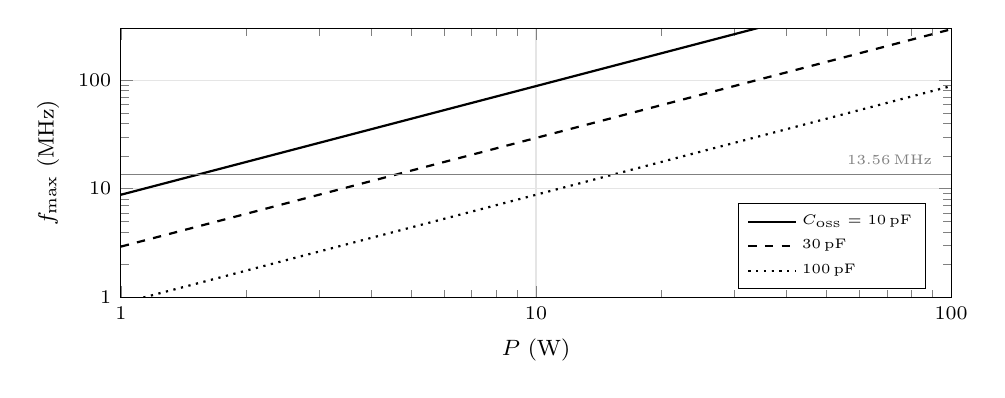
\begin{tikzpicture}
					\begin{loglogaxis}[
							width=\linewidth, height=5.0cm,
							xmin=1, xmax=100, ymin=1, ymax=300,
							xtick={1,10,100}, xticklabels={1,10,100},
							ytick={1,10,100}, yticklabels={1,10,100},
							xlabel={$P$ (W)}, ylabel={$f_\mathrm{max}$ (MHz)},
							grid=major, grid style={gray!20},
							tick label style={font=\scriptsize}, label style={font=\footnotesize},
							legend style={font=\tiny, at={(0.97,0.03)}, anchor=south east}, legend cell align=left,
						]
						\addplot[black, thick, domain=0:2, samples=2] ({10^x}, {8.802*10^x});
						\addlegendentry{$C_\mathrm{oss}=10$\,pF}
						\addplot[black, thick, dashed, domain=0:2, samples=2] ({10^x}, {2.934*10^x});
						\addlegendentry{30\,pF}
						\addplot[black, thick, dotted, domain=0:2, samples=2] ({10^x}, {0.8802*10^x});
						\addlegendentry{100\,pF}
						\addplot[gray, domain=0:2, samples=2] ({10^x}, {13.56});
						\node[font=\tiny, anchor=south east, gray] at (axis cs:95,13.56) {13.56\,MHz};
					\end{loglogaxis}
				\end{tikzpicture}
				\caption{Ideal class E at $V_\mathrm{DC}=24$\,V with $C_\mathrm{sh}=C_\mathrm{oss}$. A design point $(P,f)$ must lie below the line of its transistor}
			\end{figure}
		\end{column}
	\end{columns}
\end{frame}

%%%%%%%%%%%%%%%%%%%%%%%%%%%%%%%%%%%%%%%%%%%%%%%%%%%%%%%%%%%%%
%% Task: is 100 pF small enough %%
%%%%%%%%%%%%%%%%%%%%%%%%%%%%%%%%%%%%%%%%%%%%%%%%%%%%%%%%%%%%%
% Two pages: task (page 1) and task with solution (page 2).
\begin{frame}<handout:1-2>
	\frametitle{Is 100\,pF small enough?}
	\begin{block}{Task (3 minutes)}
		A transistor considered for B5 has an effective $C_\mathrm{oss}$ of 100\,pF at 24\,V.
		\begin{enumerate}
			\item Can it work in the 10\,W, 24\,V class E at 13.56\,MHz?
			\item Which power or which input voltage would suit it at 13.56\,MHz?
		\end{enumerate}
	\end{block}
	\onslide<2-|handout:2>{
		\begin{enumerate}
			\item $f_\mathrm{max}=0.0507\cdot10\,\mathrm{W}/(100\,\mathrm{pF}\cdot(24\,\mathrm{V})^2)=8.8$\,MHz $<13.56$\,MHz: no. $C_\mathrm{oss}$ alone exceeds the required 64.9\,pF. With $Q_\mathrm{L}=10$: 9.9\,MHz, still no.
			\item $P\geq10\,\mathrm{W}\cdot100/64.9=15.4$\,W at 24\,V, or $V_\mathrm{DC}\leq24\,\mathrm{V}\cdot\sqrt{64.9/100}=19.3$\,V at 10\,W. Otherwise a smaller transistor, or a $\Phi_2$ inverter, in which the drain capacitance is a design choice.
		\end{enumerate}
	}
\end{frame}

%%%%%%%%%%%%%%%%%%%%%%%%%%%%%%%%%%%%%%%%%%%%%%%%%%%%%%%%%%%%%
%% Load sensitivity %%
%%%%%%%%%%%%%%%%%%%%%%%%%%%%%%%%%%%%%%%%%%%%%%%%%%%%%%%%%%%%%
\begin{frame}
	\frametitle{Load sensitivity}
	\begin{columns}[T]
		\begin{column}{0.5\textwidth}
			\begin{figure}
				\centering
				\begin{tikzpicture}
					\begin{axis}[
							width=\linewidth, height=5.0cm,
							xmin=0, xmax=360, xtick={0,90,180,270,360},
							ymin=-0.2, ymax=4.4, ytick={0,1,2,3,4},
							xlabel={$\theta=\omega t$ ($^\circ$)}, ylabel={$v_\mathrm{S}/V_\mathrm{DC}$},
							grid=major, grid style={gray!20},
							tick label style={font=\scriptsize}, label style={font=\footnotesize},
							legend style={font=\tiny, at={(0.03,0.97)}, anchor=north west}, legend cell align=left,
						]
						\addplot[black, thick, dashed] table[x=th, y=v06] {fig/lec10/classe_load.dat};
						\addlegendentry{$R=0.6\,R_\mathrm{nom}$}
						\addplot[black, thick] table[x=th, y=v10] {fig/lec10/classe_load.dat};
						\addlegendentry{$R=R_\mathrm{nom}$}
						\addplot[black, thick, dotted] table[x=th, y=v16] {fig/lec10/classe_load.dat};
						\addlegendentry{$R=1.6\,R_\mathrm{nom}$}
					\end{axis}
				\end{tikzpicture}
				\caption{Switch voltage of a class E tuned for $R_\mathrm{nom}$ ($Q_\mathrm{L}=10$) and operated at three load resistances; exact steady state}
			\end{figure}
		\end{column}
		\begin{column}{0.47\textwidth}
			\footnotesize
			\begin{itemize}
				\item $R<R_\mathrm{nom}$: $v_\mathrm{S}$ reaches zero before turn-on and the body diode conducts (from $319^\circ$ at $0.6\,R_\mathrm{nom}$). The turn-on is still at zero voltage, but the peak rises to $4.07\,V_\mathrm{DC}$ ($+13$\,\%).
				\item $R>R_\mathrm{nom}$: $v_\mathrm{S}$ has not returned to zero at turn-on, $1.16\,V_\mathrm{DC}$ at $1.6\,R_\mathrm{nom}$. The switch discharges $C_\mathrm{sh}$ in its channel: $\tfrac12C_\mathrm{sh}v_\mathrm{S}^2f$ is 4.8\,\% of the output power.
				\item In wireless power the coil position changes the reflected resistance (B4). Design for the whole range, or keep the load constant with a compression or tunable network (later).
				\item Simulate with the real $C_\mathrm{oss}(v)$ before the layout.
			\end{itemize}
		\end{column}
	\end{columns}
	\blfootnote{Simulation: \texttt{lecture/sim/classe\_timedomain.py}, ideal switch with body diode, linear $C_\mathrm{sh}$.}
\end{frame}

%%%%%%%%%%%%%%%%%%%%%%%%%%%%%%%%%%%%%%%%%%%%%%%%%%%%%%%%%%%%%
%% Class Phi2 %%
%%%%%%%%%%%%%%%%%%%%%%%%%%%%%%%%%%%%%%%%%%%%%%%%%%%%%%%%%%%%%
\subsection{\texorpdfstring{Class $\Phi_2$ and class DE}{Class Phi2 and class DE}}

\begin{frame}
	\frametitle{The class $\Phi_2$ inverter}
	\begin{columns}[T]
		\begin{column}{0.52\textwidth}
			\begin{figure}
				\centering
				\begin{circuitikz}[scale=0.74, transform shape]
					\draw (0,0) to[V, l=$V_\mathrm{in}$] (0,3.6) to[L, l=$L_\mathrm{F}$] (2.4,3.6) node[circ]{};
					\draw (2.4,3.6) -- (2.4,2.9) node[nigfete, anchor=D] (S) {};
					\draw (S.S) -- (2.4,0) node[circ]{};
					\draw (2.4,3.6) -- (3.7,3.6) to[C, l=$C_\mathrm{F}$, v_>=$v_\mathrm{S}$] (3.7,0) node[circ]{};
					\draw (3.7,3.6) -- (5.0,3.6) node[circ]{} to[L, l=$L_\mathrm{MR}$] (5.0,1.8) to[C, l=$C_\mathrm{MR}$] (5.0,0) node[circ]{};
					\draw (5.0,3.6) to[C, l=$C_\mathrm{S}$] (6.6,3.6) to[L, l=$L_\mathrm{S}$] (8.4,3.6) to[R, l=$R$] (8.4,0) -- (0,0);
				\end{circuitikz}
				\caption{Class $\Phi_2$ inverter; $C_\mathrm{F}$ includes $C_\mathrm{oss}$; $L_\mathrm{S}$, $C_\mathrm{S}$: output network to the load $R$}
			\end{figure}
		\end{column}
		\begin{column}{0.46\textwidth}
			\footnotesize
			\begin{itemize}
				\item $L_\mathrm{MR}$ and $C_\mathrm{MR}$ are series resonant near $2f_\mathrm{s}$ ($f_\mathrm{s}$: switching frequency): they short the drain at the second harmonic.
				\item Together with $L_\mathrm{F}$ and $C_\mathrm{F}$ the drain network has impedance peaks at $f_\mathrm{s}$ and $3f_\mathrm{s}$, like a shorted quarter-wave line.
				\item Fundamental plus third harmonic make $v_\mathrm{S}$ nearly trapezoidal: measured peak about $2.4\,V_\mathrm{in}$ (class E: $3.56\,V_\mathrm{DC}$).
				\item $L_\mathrm{F}$ is a small resonant element, not a bulk choke: little stored energy, so the inverter starts and stops within a few periods.
				\item Prototype of Rivas et al.: 30\,MHz, over 500\,W, drain efficiency above 92\,\%, duty ratio $D=0.3$.
			\end{itemize}
		\end{column}
	\end{columns}
	\blfootnote{Source: J.\,M. Rivas et al., IEEE Trans.\ Power Electron., vol.\ 23, no.\ 4, 2008.}
\end{frame}

%%%%%%%%%%%%%%%%%%%%%%%%%%%%%%%%%%%%%%%%%%%%%%%%%%%%%%%%%%%%%
%% Tuning the Phi2 network %%
%%%%%%%%%%%%%%%%%%%%%%%%%%%%%%%%%%%%%%%%%%%%%%%%%%%%%%%%%%%%%
\begin{frame}
	\frametitle{Tuning the $\Phi_2$ network}
	\begin{columns}[T]
		\begin{column}{0.5\textwidth}
			\footnotesize
			Step 1: $L_\mathrm{MR}C_\mathrm{MR}=1/(4\omega_\mathrm{s}^2)$, series resonance at $2\omega_\mathrm{s}$. Admittance of the drain network:
			\begin{equation*}
				Y=\mathrm{j}\left[\omega C_\mathrm{F}-\frac{1}{\omega L_\mathrm{F}}+\frac{\omega C_\mathrm{MR}}{1-\omega^2/(4\omega_\mathrm{s}^2)}\right]
			\end{equation*}
			Step 2: $Y=0$ (impedance peak) at $\omega_\mathrm{s}$ and at $3\omega_\mathrm{s}$ gives
			\begin{equation*}
				C_\mathrm{MR}=\frac{15}{16}C_\mathrm{F},\quad L_\mathrm{F}=\frac{4}{9\,\omega_\mathrm{s}^2C_\mathrm{F}},\quad L_\mathrm{MR}=\frac{4}{15\,\omega_\mathrm{s}^2C_\mathrm{F}}
			\end{equation*}
			\begin{itemize}
				\item Example, 30\,MHz and $C_\mathrm{F}=20$\,pF: $L_\mathrm{F}=625$\,nH, $C_\mathrm{MR}=18.8$\,pF, $L_\mathrm{MR}=375$\,nH.
				\item Step 3: extra drain capacitance lowers the $3f_\mathrm{s}$ peak by 4 to 8\,dB, which lowers the peak voltage; a smaller $L_\mathrm{F}$ makes the drain impedance $Z_\mathrm{ds}(f_\mathrm{s})$ inductive by 30 to $60^\circ$ for ZVS.
			\end{itemize}
		\end{column}
		\begin{column}{0.47\textwidth}
			\begin{figure}
				\centering
				\begin{tikzpicture}
					\begin{loglogaxis}[
							width=\linewidth, height=4.6cm,
							xmin=0.2, xmax=5, ymin=0.1, ymax=100,
							xtick={0.2,0.5,1,2,3,5}, xticklabels={0.2,0.5,1,2,3,5},
							ytick={0.1,1,10,100}, yticklabels={0.1,1,10,100},
							xlabel={$f/f_\mathrm{s}$}, ylabel={$|Z|\,\omega_\mathrm{s}C_\mathrm{F}$},
							grid=major, grid style={gray!20},
							tick label style={font=\scriptsize}, label style={font=\footnotesize},
							legend style={font=\tiny, at={(0.5,1.07)}, anchor=south, legend columns=2, /tikz/every even column/.append style={column sep=0.25cm}}, legend cell align=left,
						]
						\addplot[black, thick] table[x=F, y=Z] {fig/lec10/phi2_z.dat};
						\addlegendentry{$\Phi_2$ network}
						\addplot[black, dashed] table[x=F, y=Zc] {fig/lec10/phi2_z.dat};
						\addlegendentry{$C_\mathrm{F}$ alone}
					\end{loglogaxis}
				\end{tikzpicture}
				\caption{Normalised impedance of the drain network $L_\mathrm{F}\,\|\,C_\mathrm{F}\,\|\,(L_\mathrm{MR}+C_\mathrm{MR})$ after step 2, inductor $Q=100$}
			\end{figure}
		\end{column}
	\end{columns}
	\blfootnote{Tuning procedure after Rivas et al., 2008.}
\end{frame}

%%%%%%%%%%%%%%%%%%%%%%%%%%%%%%%%%%%%%%%%%%%%%%%%%%%%%%%%%%%%%
%% Class D and DE %%
%%%%%%%%%%%%%%%%%%%%%%%%%%%%%%%%%%%%%%%%%%%%%%%%%%%%%%%%%%%%%
\begin{frame}
	\frametitle{Class D and DE at 6.78\,MHz}
	\begin{columns}[T]
		\begin{column}{0.48\textwidth}
			\begin{figure}
				\centering
				\begin{circuitikz}[scale=0.74, transform shape]
					\draw (0,0) to[V, l=$V_\mathrm{DC}$] (0,4) -- (1.8,4) node[nigfete, anchor=D] (S1) {};
					\draw (0,0) -- (1.8,0) node[nigfete, anchor=S] (S2) {};
					\draw (S1.S) -- (S2.D);
					\coordinate (m) at ($(S1.S)!0.5!(S2.D)$);
					\draw (m) node[circ]{} -- ++(0.6,0) to[L, l=$L_\mathrm{r}$] ++(1.8,0) to[C, l=$C_\mathrm{r}$] ++(1.6,0) coordinate (b);
					\draw (b) to[R, l=$R$] (b |- 0,0) -- (1.8,0);
				\end{circuitikz}
				\caption{Half-bridge with series-resonant load}
			\end{figure}
		\end{column}
		\begin{column}{0.5\textwidth}
			\footnotesize
			\begin{itemize}
				\item Each switch blocks only $V_\mathrm{DC}$: the lowest voltage stress of all inverters (class E: $3.56\,V_\mathrm{DC}$).
				\item ZVS class D (L8): driven above resonance, the lagging tank current recharges the $C_\mathrm{oss}$ of both switches in the dead time. Class DE: each switch is on for less than half the period; shunt capacitance and dead time give ZVS and zero $\mathrm{d}v/\mathrm{d}t$ at turn-on, as in class E.
				\item The price: a high-side switch, with drive and timing as in any half-bridge. Feasible at 6.78\,MHz with GaN (half period 73.7\,ns).
				\item The fundamental of the square wave, amplitude $2V_\mathrm{DC}/\pi$, drives $R$: $P=2V_\mathrm{DC}^2/(\pi^2R)$. Brief B4 (24\,V, 15\,W): class D needs $R=7.8\,\Omega$, 24\,V across each switch; class E needs $R=22.1\,\Omega$, 85\,V peak.
			\end{itemize}
		\end{column}
	\end{columns}
	\blfootnote{Sources: Kazimierczuk and Czarkowski, 2011; H. Sekiya et al., IEEE Trans.\ Power Electron., vol.\ 30, no.\ 7, 2015 (class DE at any duty ratio).}
\end{frame}

%%%%%%%%%%%%%%%%%%%%%%%%%%%%%%%%%%%%%%%%%%%%%%%%%%%%%%%%%%%%%
%% Choosing the inverter %%
%%%%%%%%%%%%%%%%%%%%%%%%%%%%%%%%%%%%%%%%%%%%%%%%%%%%%%%%%%%%%
\begin{frame}
	\frametitle{Choosing the inverter}
	\begin{table}
		\centering
		\scriptsize
		\begin{tabular}{|l|>{\raggedright\arraybackslash}p{3.4cm}|>{\raggedright\arraybackslash}p{3.4cm}|>{\raggedright\arraybackslash}p{3.4cm}|}
			\hline
			                     & \textbf{Class D/DE}                 & \textbf{Class E}                              & \textbf{Class $\Phi_2$}                   \\
			\hline
			Switches             & two, one high side                  & one, ground-referenced                        & one, ground-referenced                    \\
			Peak switch voltage  & $V_\mathrm{DC}$                     & $3.56\,V_\mathrm{DC}$, more with $C_\mathrm{oss}(v)$ & about $2.4\,V_\mathrm{in}$ (measured) \\
			Input inductor       & none                                & bulk choke $L_\mathrm{F}$                     & small resonant $L_\mathrm{F}$             \\
			$C_\mathrm{oss}$     & charged in the dead time            & fixes $f_\mathrm{max}$ for given $P$          & part of $C_\mathrm{F}$, which is chosen freely             \\
			Soft switching       & ZVS with inductive tank; DE: ZVS and ZDS & ZVS and ZDS near $R_\mathrm{nom}$ only   & ZVS by tuning of $Z_\mathrm{ds}$          \\
			Typical use          & WPT at 6.78\,MHz, RF generators     & RF amplifiers, WPT, VHF dc--dc                & VHF dc--dc with on/off control            \\
			\hline
		\end{tabular}
		\caption{Single-ended and half-bridge resonant inverters for 6.78 to 30\,MHz}
	\end{table}
	\begin{block}{Key message}
		Low input voltage and a wide load range favour class DE; high voltage, one switch and fast on/off control favour $\Phi_2$; class E is the simplest and the reference.
	\end{block}
	\blfootnote{Sources: Rivas et al., 2008; Kazimierczuk, 2014.}
\end{frame}

%%%%%%%%%%%%%%%%%%%%%%%%%%%%%%%%%%%%%%%%%%%%%%%%%%%%%%%%%%%%%
%% Resonant rectifiers %%
%%%%%%%%%%%%%%%%%%%%%%%%%%%%%%%%%%%%%%%%%%%%%%%%%%%%%%%%%%%%%
\subsection{Rectifiers and matching}

\begin{frame}
	\frametitle{Resonant rectifiers}
	\begin{columns}[T]
		\begin{column}{0.5\textwidth}
			\begin{figure}
				\centering
				\begin{circuitikz}[scale=0.74, transform shape]
					\draw (0,3) node[ocirc]{} to[C, l=$C_\mathrm{S}$, i>^=$i_\mathrm{in}$] (2,3) node[circ]{};
					\draw (2,3) to[L, l_=$L_\mathrm{R}$] (2,0) node[circ]{};
					\draw (2,3) -- (3,3) node[circ]{} to[D, l_=$D$] (5,3) node[circ]{};
					\draw (3,3) -- (3,4.2) to[C, l=$C_\mathrm{D}$] (5,4.2) -- (5,3);
					\draw (5,3) -- (6.2,3) to[C, l=$C_\mathrm{o}$] (6.2,0) node[circ]{};
					\draw (6.2,3) -- (7.6,3) to[R, l=$R_\mathrm{L}$] (7.6,0) -- (0,0) node[ocirc]{};
				\end{circuitikz}
				\caption{Resonant half-wave rectifier; $C_\mathrm{D}$ includes the junction capacitance; $C_\mathrm{S}$ blocks DC}
			\end{figure}
		\end{column}
		\begin{column}{0.47\textwidth}
			\footnotesize
			\begin{itemize}
				\item At VHF the junction capacitance of the diode is comparable with the tank capacitors. The resonant rectifier makes it part of the tank: $C_\mathrm{D}$ resonates with $L_\mathrm{R}$ while the diode is off.
				\item The diode voltage thus changes slowly, with little ringing. Schottky diodes (Si or SiC) add no recovery spike.
				\item The inverter sees the rectifier as $R_\mathrm{rec}+\mathrm{j}X_\mathrm{rec}$ at the fundamental. It changes with output voltage and power, as the conduction angle of the diode changes; the constant $8R_\mathrm{L}/\pi^2$ of L9 does not apply.
				\item Inverter and rectifier must be tuned together, by simulation over the operating range.
			\end{itemize}
		\end{column}
	\end{columns}
	\blfootnote{Sources: Perreault et al., APEC 2009; Kazimierczuk and Czarkowski, 2011 (class E rectifiers).}
\end{frame}

%%%%%%%%%%%%%%%%%%%%%%%%%%%%%%%%%%%%%%%%%%%%%%%%%%%%%%%%%%%%%
%% Resistance compression %%
%%%%%%%%%%%%%%%%%%%%%%%%%%%%%%%%%%%%%%%%%%%%%%%%%%%%%%%%%%%%%
\begin{frame}
	\frametitle{Resistance compression}
	{\small Class E and $\Phi_2$ inverters need a nearly constant load, but the resistance $R$ of a rectifier changes with power and output voltage.}
	\begin{columns}[T]
		\begin{column}{0.5\textwidth}
			\begin{figure}
				\centering
				\begin{circuitikz}[scale=0.6, transform shape]
					\draw (0,1.6) node[ocirc]{} node[left]{$Z_\mathrm{in}$} -- (1,1.6) node[circ]{};
					\draw (1,1.6) |- (1.6,2.7) to[L, l=$+\mathrm{j}X$] (3.6,2.7) to[R, l=$R$] (5.6,2.7) node[ground]{};
					\draw (1,1.6) |- (1.6,0.5) to[C, l=$-\mathrm{j}X$] (3.6,0.5) to[R, l=$R$] (5.6,0.5) node[ground]{};
				\end{circuitikz}
				\caption{Two identical rectifiers $R$, fed via $\pm\mathrm{j}X$}
			\end{figure}
			\vspace{-0.4cm}
			\footnotesize
			\begin{align*}
				Y_\mathrm{in} & =\frac{1}{R+\mathrm{j}X}+\frac{1}{R-\mathrm{j}X}=\frac{2R}{R^2+X^2} \\
				Z_\mathrm{in} & =\frac{X}{2}\left(\frac{R}{X}+\frac{X}{R}\right)
			\end{align*}
		\end{column}
		\begin{column}{0.47\textwidth}
			\begin{figure}
				\centering
				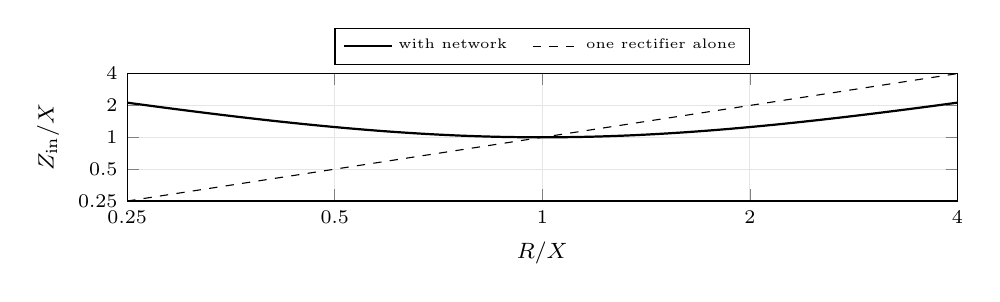
\begin{tikzpicture}
					\begin{loglogaxis}[
							width=\linewidth, height=3.2cm,
							xmin=0.25, xmax=4, ymin=0.25, ymax=4,
							xtick={0.25,0.5,1,2,4}, xticklabels={0.25,0.5,1,2,4},
							ytick={0.25,0.5,1,2,4}, yticklabels={0.25,0.5,1,2,4},
							xlabel={$R/X$}, ylabel={$Z_\mathrm{in}/X$},
							grid=major, grid style={gray!20},
							tick label style={font=\scriptsize}, label style={font=\footnotesize},
							legend style={font=\tiny, at={(0.5,1.07)}, anchor=south, legend columns=2, /tikz/every even column/.append style={column sep=0.25cm}}, legend cell align=left,
						]
						\addplot[black, thick, domain=-0.6021:0.6021, samples=81] ({10^x}, {(10^x+10^(-x))/2});
						\addlegendentry{with network}
						\addplot[black, dashed, domain=-0.6021:0.6021, samples=2] ({10^x}, {10^x});
						\addlegendentry{one rectifier alone}
					\end{loglogaxis}
				\end{tikzpicture}
				\caption{Input impedance, resistive for any $R$}
			\end{figure}
			\vspace{-0.3cm}
			{\small Example: $R$ varies 4:1, from $X/2$ to $2X$; $Z_\mathrm{in}$ varies only 1.25:1, from $X$ to $1.25X$.}
		\end{column}
	\end{columns}
	\blfootnote{Source: Y. Han, O. Leitermann, D.\,A. Jackson, J.\,M. Rivas, D.\,J. Perreault, IEEE Trans.\ Power Electron., vol.\ 22, no.\ 1, 2007.}
\end{frame}

%%%%%%%%%%%%%%%%%%%%%%%%%%%%%%%%%%%%%%%%%%%%%%%%%%%%%%%%%%%%%
%% L-section matching %%
%%%%%%%%%%%%%%%%%%%%%%%%%%%%%%%%%%%%%%%%%%%%%%%%%%%%%%%%%%%%%
\begin{frame}
	\frametitle{L-section matching}
	\begin{columns}[T]
		\begin{column}{0.47\textwidth}
			\begin{figure}
				\centering
				\begin{circuitikz}[scale=0.74, transform shape]
					\draw (0,2.4) node[ocirc]{} -- (1.4,2.4) node[circ]{} to[L, l=$X_\mathrm{s}$] (3.8,2.4) to[R, l=$R_\mathrm{low}$] (3.8,0) -- (0,0) node[ocirc]{};
					\draw (1.4,2.4) to[C, l_=$X_\mathrm{p}$] (1.4,0) node[circ]{};
					\draw[->] (-0.9,1.2) node[left, align=center]{input:\\$R_\mathrm{high}$} -- (-0.2,1.2);
				\end{circuitikz}
				\caption{Low-pass L-section: the load $R_\mathrm{low}$ appears as $R_\mathrm{high}$ at the input. Shunt element on the high side, series element on the low side}
			\end{figure}
		\end{column}
		\begin{column}{0.5\textwidth}
			\footnotesize
			Seen from the shunt element, $R_\mathrm{low}+\mathrm{j}X_\mathrm{s}$ equals $R_\mathrm{low}(1+Q^2)$ in parallel with a reactance $R_\mathrm{high}/Q$, where $Q=X_\mathrm{s}/R_\mathrm{low}$. Choose $R_\mathrm{low}(1+Q^2)=R_\mathrm{high}$; $X_\mathrm{p}$ cancels the reactance:
			\begin{equation*}
				Q=\sqrt{\frac{R_\mathrm{high}}{R_\mathrm{low}}-1},\quad X_\mathrm{s}=QR_\mathrm{low},\quad X_\mathrm{p}=\frac{R_\mathrm{high}}{Q}
			\end{equation*}
			Each element carries the reactive power $QP$; with the quality factors $Q_\mathrm{ind}$, $Q_\mathrm{cap}$ of the parts: $\eta\approx1-Q/Q_\mathrm{ind}-Q/Q_\mathrm{cap}$.
		\end{column}
	\end{columns}
	\footnotesize
	\begin{itemize}
		\item The high-pass version (series C, shunt L) follows the same equations. The low-pass version also filters harmonics; the high-pass version blocks DC.
		\item A larger ratio $R_\mathrm{high}/R_\mathrm{low}$ needs a larger $Q$: narrower bandwidth, more loss. The inductor dominates the loss ($Q_\mathrm{ind}\approx100$ to 300; C0G: $Q_\mathrm{cap}>1000$).
	\end{itemize}
	\blfootnote{Sources: Y. Han, D.\,J. Perreault, IEEE Trans.\ Power Electron., vol.\ 21, no.\ 5, 2006; D.\,J. Perreault, MIT 6.622, Lecture 37, 2023.}
\end{frame}

%%%%%%%%%%%%%%%%%%%%%%%%%%%%%%%%%%%%%%%%%%%%%%%%%%%%%%%%%%%%%
%% Task: L-match 50 to 5 ohm %%
%%%%%%%%%%%%%%%%%%%%%%%%%%%%%%%%%%%%%%%%%%%%%%%%%%%%%%%%%%%%%
% Two pages: task (page 1) and task with solution (page 2).
\begin{frame}<handout:1-2>
	\frametitle{From 50 to 5\,$\Omega$}
	\begin{block}{Task (4 minutes)}
		A 50\,$\Omega$ RF generator shall drive a 5\,$\Omega$ load at 13.56\,MHz.
		\begin{enumerate}
			\item Design a low-pass L-section: which element sits next to the load, and which values?
			\item Efficiency with $Q_\mathrm{ind}=150$ and $Q_\mathrm{cap}=1000$? Loss at 100\,W?
		\end{enumerate}
	\end{block}
	\onslide<2-|handout:2>{
		\begin{enumerate}
			\item $Q=\sqrt{50/5-1}=3$. Series inductor next to the 5\,$\Omega$ load: $X_\mathrm{s}=15\,\Omega$, $L=176$\,nH. Shunt capacitor at the 50\,$\Omega$ side: $X_\mathrm{p}=16.7\,\Omega$, $C=704$\,pF. Check: $(5+\mathrm{j}15)\,\Omega\,\|\,(-\mathrm{j}16.7\,\Omega)=50\,\Omega$.
			\item $\eta\approx1-3/150-3/1000=97.7$\,\%: 2.3\,W at 100\,W, 2\,W of it in the 176\,nH coil.
		\end{enumerate}
	}
\end{frame}

%%%%%%%%%%%%%%%%%%%%%%%%%%%%%%%%%%%%%%%%%%%%%%%%%%%%%%%%%%%%%
%% Networks with more elements %%
%%%%%%%%%%%%%%%%%%%%%%%%%%%%%%%%%%%%%%%%%%%%%%%%%%%%%%%%%%%%%
\begin{frame}
	\frametitle{Networks with more elements}
	\begin{columns}[T]
		\begin{column}{0.5\textwidth}
			\begin{figure}
				\centering
				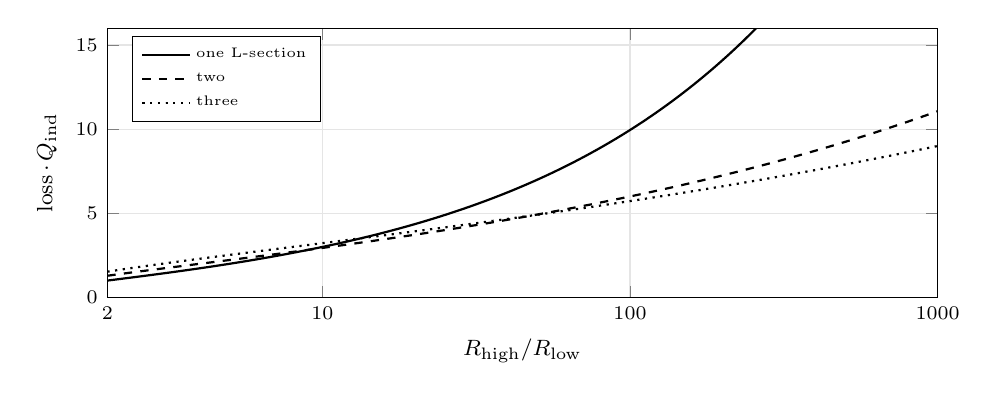
\begin{tikzpicture}
					\begin{semilogxaxis}[
							width=\linewidth, height=5.0cm,
							xmin=2, xmax=1000, ymin=0, ymax=16,
							xtick={2,10,100,1000}, xticklabels={2,10,100,1000},
							xlabel={$R_\mathrm{high}/R_\mathrm{low}$}, ylabel={loss$\,\cdot\,Q_\mathrm{ind}$},
							grid=major, grid style={gray!20},
							tick label style={font=\scriptsize}, label style={font=\footnotesize},
							legend style={font=\tiny, at={(0.03,0.97)}, anchor=north west}, legend cell align=left,
						]
						\addplot[black, thick, domain=0.30103:3, samples=120] ({10^x}, {sqrt(10^x-1)});
						\addlegendentry{one L-section}
						\addplot[black, thick, dashed, domain=0.30103:3, samples=120] ({10^x}, {2*sqrt(10^(x/2)-1)});
						\addlegendentry{two}
						\addplot[black, thick, dotted, domain=0.30103:3, samples=120] ({10^x}, {3*sqrt(10^(x/3)-1)});
						\addlegendentry{three}
					\end{semilogxaxis}
				\end{tikzpicture}
				\caption{Inductor loss (relative, times $Q_\mathrm{ind}$) of one, two and three cascaded L-sections with equal ratio per stage}
			\end{figure}
		\end{column}
		\begin{column}{0.47\textwidth}
			\small
			\begin{itemize}
				\item $N$ cascaded L-sections share the total ratio $r=R_\mathrm{high}/R_\mathrm{low}$, each transforming by $r^{1/N}$: relative loss $\approx N\sqrt{r^{1/N}-1}/Q_\mathrm{ind}$.
				\item Loss$\,\cdot\,Q_\mathrm{ind}$ for one/two/three stages: $r=10$: 3.0/2.9, no gain. $r=25$: 4.9/4.0, worthwhile. $r=100$: 9.9/6.0/5.7.
				\item The lower $Q$ per stage also widens the bandwidth.
				\item $\pi$ and T networks add a third element to set the loaded $Q$ (bandwidth, harmonic filtering) independently of the ratio; for the same ratio they have more circulating current and loss than an L-section.
			\end{itemize}
		\end{column}
	\end{columns}
	\blfootnote{Source: Han and Perreault, 2006 (optimum number of stages).}
\end{frame}

%%%%%%%%%%%%%%%%%%%%%%%%%%%%%%%%%%%%%%%%%%%%%%%%%%%%%%%%%%%%%
%% VHF dc-dc converter %%
%%%%%%%%%%%%%%%%%%%%%%%%%%%%%%%%%%%%%%%%%%%%%%%%%%%%%%%%%%%%%
\subsection{VHF dc--dc and applications}

\begin{frame}
	\frametitle{A VHF dc--dc converter}
	\begin{figure}
		\centering
		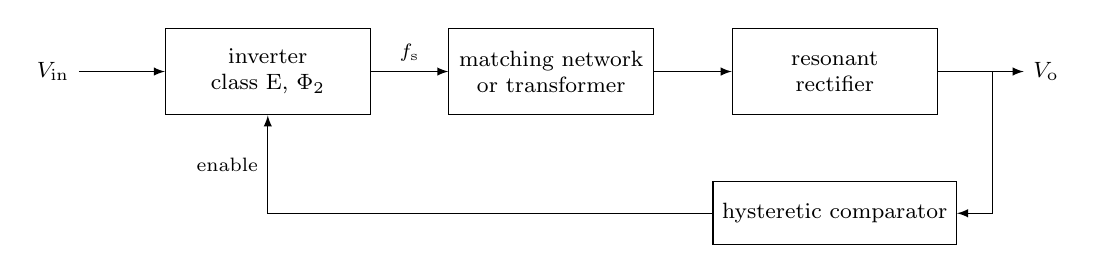
\begin{tikzpicture}[font=\footnotesize, >=latex]
			\node[draw, minimum width=2.6cm, minimum height=1.1cm, align=center] (inv) at (0,0) {inverter\\class E, $\Phi_2$};
			\node[draw, minimum width=2.6cm, minimum height=1.1cm, align=center] (mn) at (3.6,0) {matching network\\or transformer};
			\node[draw, minimum width=2.6cm, minimum height=1.1cm, align=center] (rec) at (7.2,0) {resonant\\rectifier};
			\node[draw, minimum width=2.4cm, minimum height=0.8cm, align=center] (cmp) at (7.2,-1.8) {hysteretic comparator};
			\draw[->] (-2.4,0) node[left]{$V_\mathrm{in}$} -- (inv.west);
			\draw[->] (inv) -- node[above, font=\scriptsize]{$f_\mathrm{s}$} (mn);
			\draw[->] (mn) -- (rec);
			\draw[->] (rec.east) -- (9.6,0) node[right]{$V_\mathrm{o}$};
			\draw[->] (9.2,0) |- (cmp.east);
			\draw[->] (cmp.west) -| node[pos=0.75, left, font=\scriptsize]{enable} (inv.south);
		\end{tikzpicture}
		\caption{Energy conversion at $f_\mathrm{s}$, regulation by switching the whole converter on and off}
	\end{figure}
	\vspace{-0.2cm}
	\footnotesize
	\begin{itemize}
		\item PWM within the period is impractical. Frequency or phase control would keep the converter running at light load, where the resonant and gate-drive losses stay while the power falls.
		\item Instead the power stage always runs at its design point. A hysteretic comparator switches it on and off, at a modulation frequency far below $f_\mathrm{s}$, and holds $V_\mathrm{o}$ between two thresholds. Losses occur only while it runs.
		\item This needs a converter with little stored energy (no bulk choke) that starts and stops within a few periods. The input and output capacitors are sized for the modulation frequency, not for $f_\mathrm{s}$.
	\end{itemize}
	\blfootnote{Source: Perreault et al., APEC 2009.}
\end{frame}

%%%%%%%%%%%%%%%%%%%%%%%%%%%%%%%%%%%%%%%%%%%%%%%%%%%%%%%%%%%%%
%% On/off control %%
%%%%%%%%%%%%%%%%%%%%%%%%%%%%%%%%%%%%%%%%%%%%%%%%%%%%%%%%%%%%%
\begin{frame}
	\frametitle{On/off control}
	\begin{columns}[T]
		\begin{column}{0.46\textwidth}
			\begin{figure}
				\centering
				\begin{tikzpicture}
					\begin{groupplot}[
							group style={group size=1 by 2, vertical sep=0.25cm, xticklabels at=edge bottom},
							width=\linewidth, height=2.9cm,
							xmin=0, xmax=9, xtick=\empty,
							tick label style={font=\scriptsize}, label style={font=\footnotesize},
						]
						\nextgroupplot[ymin=0.3, ymax=0.78, ytick={0.4,0.6}, yticklabels={$V_\mathrm{L}$,$V_\mathrm{H}$}, ylabel={$v_\mathrm{o}$}]
						\addplot[gray, dashed, domain=0:9, samples=2] {0.4};
						\addplot[gray, dashed, domain=0:9, samples=2] {0.6};
						\addplot[black, thick] coordinates {(0,0.4) (1,0.6) (3.5,0.4) (4.5,0.6) (7,0.4) (8,0.6) (9,0.52)};
						\node[font=\tiny, anchor=south west, inner sep=1pt] at (axis cs:1.2,0.61) {off: the load discharges $C_\mathrm{o}$};
						\nextgroupplot[ymin=-0.2, ymax=1.3, ytick={0,1}, yticklabels={off,on}, ylabel={enable}, xlabel={time}]
						\addplot[black, thick, const plot] coordinates {(0,1) (1,0) (3.5,1) (4.5,0) (7,1) (8,0) (9,0)};
					\end{groupplot}
				\end{tikzpicture}
				\caption{Hysteretic on/off control (sketch): enabled, the converter delivers full power and $v_\mathrm{o}$ rises to $V_\mathrm{H}$; then it stops until $v_\mathrm{o}$ has fallen to $V_\mathrm{L}$. On-time fraction = load power / full power}
			\end{figure}
		\end{column}
		\begin{column}{0.51\textwidth}
			\footnotesize
			Resonant and PWM boost converter for the same task, 11 to 16\,V in, 32.4\,V and up to 18\,W out:
			\begin{table}
				\centering
				\scriptsize
				\begin{tabular}{|l|c|c|}
					\hline
					                            & resonant                 & PWM                    \\
					                            & 110\,MHz                 & 500\,kHz               \\
					\hline
					efficiency at 5--100\,\% load & 81--87\,\%             & 74--89\,\%             \\
					largest inductor            & 33\,nH, air              & 10\,$\mu$H             \\
					magnetics volume (relative) & $<1/4$                   & 1                      \\
					output ripple               & 200\,mV$_\mathrm{pp}$    & 10\,mV$_\mathrm{pp}$   \\
					\hline
				\end{tabular}
			\end{table}
			\vspace{-0.3cm}
			\begin{itemize}
				\item At light load the resonant converter keeps its efficiency: it runs at its design point, and only for the fraction of time the load needs.
				\item The price: output ripple at the modulation frequency (200 against 10\,mV) and an EMI spectrum spread by the varying modulation.
			\end{itemize}
		\end{column}
	\end{columns}
	\blfootnote{Sources: Perreault et al., APEC 2009; R.\,C.\,N. Pilawa-Podgurski et al., IEEE Trans.\ Power Electron., vol.\ 24, no.\ 6, 2009.}
\end{frame}

%%%%%%%%%%%%%%%%%%%%%%%%%%%%%%%%%%%%%%%%%%%%%%%%%%%%%%%%%%%%%
%% Wireless power transfer %%
%%%%%%%%%%%%%%%%%%%%%%%%%%%%%%%%%%%%%%%%%%%%%%%%%%%%%%%%%%%%%
\begin{frame}
	\frametitle{Wireless power transfer}
	\begin{columns}[T]
		\begin{column}{0.5\textwidth}
			\begin{figure}
				\centering
				\begin{circuitikz}[scale=0.7, transform shape]
					\draw (0,0) to[sV, l=$V_1$] (0,2.6) to[C, l=$C_1$] (1.6,2.6) to[R, l=$R_1$] (3.0,2.6) to[L, l_=$L_1$] (3.0,0) -- (0,0);
					\draw (4.2,0) to[L, l_=$L_2$] (4.2,2.6) to[R, l=$R_2$] (5.6,2.6) to[C, l=$C_2$] (7.0,2.6) to[R, l=$R_\mathrm{L}$] (7.0,0) -- (4.2,0);
					\draw[<->] (3.3,1.3) -- node[above]{$M$} (3.9,1.3);
				\end{circuitikz}
				\caption{Series-compensated inductive link: $C_1$, $C_2$ resonate with $L_1$, $L_2$; coupling factor $k=M/\sqrt{L_1L_2}$}
			\end{figure}
			\vspace{-0.3cm}
			\footnotesize
			$R_1$, $R_2$: coil resistances; $Q_i=\omega L_i/R_i$: coil quality factors; $U=k\sqrt{Q_1Q_2}$: figure of merit of the link. The efficiency is highest for $R_\mathrm{L}=R_2\sqrt{1+U^2}$:
			\begin{equation*}
				\eta_\mathrm{max}=\frac{U^2}{\left(1+\sqrt{1+U^2}\right)^2}
			\end{equation*}
		\end{column}
		\begin{column}{0.47\textwidth}
			\begin{figure}
				\centering
				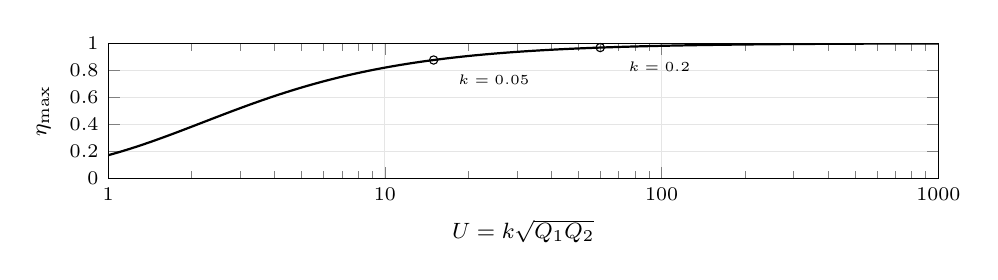
\begin{tikzpicture}
					\begin{semilogxaxis}[
							width=\linewidth, height=3.3cm,
							xmin=1, xmax=1000, ymin=0, ymax=1,
							xtick={1,10,100,1000}, xticklabels={1,10,100,1000},
							xlabel={$U=k\sqrt{Q_1Q_2}$}, ylabel={$\eta_\mathrm{max}$},
							grid=major, grid style={gray!20},
							tick label style={font=\scriptsize}, label style={font=\footnotesize},
						]
						\addplot[black, thick, domain=0:3, samples=120] ({10^x}, {(10^x)^2/(1+sqrt(1+(10^x)^2))^2});
						\addplot[only marks, mark=o, mark size=1.5pt] coordinates {(15,0.8753) (60,0.9672)};
						\node[font=\tiny, anchor=north west] at (axis cs:17,0.84) {$k=0.05$};
						\node[font=\tiny, anchor=north west] at (axis cs:70,0.93) {$k=0.2$};
					\end{semilogxaxis}
				\end{tikzpicture}
				\caption{Highest link efficiency against $U$; marks: $Q_1=Q_2=300$ with $k=0.05$ (87.5\,\%) and $k=0.2$ (96.7\,\%)}
			\end{figure}
			\vspace{-0.4cm}
			\footnotesize
			Coil $Q$ rises with frequency up to the self-resonance; a loosely coupled link (small $k$) therefore works at MHz. AirFuel Resonant uses the 6.78\,MHz ISM band (IEC 63028:2017). The inverter sees an impedance that changes with $k$ and load (B4).
		\end{column}
	\end{columns}
	\blfootnote{Derivation in Tutorial 10; e.g.\ R. Bosshard et al., IEEE JESTPE, vol.\ 3, no.\ 1, 2015 (coil optimisation with $kQ$).}
\end{frame}

%%%%%%%%%%%%%%%%%%%%%%%%%%%%%%%%%%%%%%%%%%%%%%%%%%%%%%%%%%%%%
%% Industrial RF power %%
%%%%%%%%%%%%%%%%%%%%%%%%%%%%%%%%%%%%%%%%%%%%%%%%%%%%%%%%%%%%%
\begin{frame}
	\frametitle{Industrial RF power}
	\begin{columns}[T]
		\begin{column}{0.47\textwidth}
			\footnotesize
			\begin{itemize}
				\item Plasma processing of semiconductors runs mostly at 13.56\,MHz. The plasma impedance changes with gas, pressure and power; the generator expects 50\,$\Omega$.
				\item Matching networks tuned by motor-driven vacuum capacitors are slow; switched-mode tunable matching networks adjust electronically and faster.
				\item In an ISM band the fundamental is exempt from the emission limits: 6.765 to 6.795, 13.553 to 13.567, 26.957 to 27.283, 40.66 to 40.70\,MHz (ITU Radio Regulations). Harmonics and spurious emissions must meet CISPR 11.
			\end{itemize}
		\end{column}
		\begin{column}{0.5\textwidth}
			\begin{table}
				\centering
				\scriptsize
				\begin{tabular}{|>{\raggedright\arraybackslash}p{3.6cm}|>{\raggedright\arraybackslash}p{2.0cm}|}
					\hline
					\textbf{System}                                                   & \textbf{Group}            \\
					\hline
					5\,kW, 13.56\,MHz inverter, wide power range                      & Zhang, MIT, 2022          \\
					1\,kW, 13.56\,MHz inverter, 95.4\,\%                              & Braun, MIT, 2019          \\
					1.5\,kW, 13.56\,MHz tunable matching network, $2-\mathrm{j}15\,\Omega$ to 50\,$\Omega$ & Al Bastami et al., 2020 \\
					1\,kW, 6.78\,MHz inductive WPT, 95\,\%                            & Gu, Rivas, Stanford, 2021 \\
					3.7\,kW, 13.56\,MHz capacitive WPT, 93\,\%                        & Regensberger, Cornell, 2022 \\
					\hline
				\end{tabular}
				\caption{Examples collected by Perreault (APEC 2024 plenary)}
			\end{table}
		\end{column}
	\end{columns}
	\blfootnote{Sources: D.\,J. Perreault, ``Opportunities, progress and challenges in high-frequency power conversion,'' plenary, IEEE APEC 2024; A. Al Bastami et al., IEEE Open J.\ Power Electron., vol.\ 1, 2020.}
\end{frame}

%%%%%%%%%%%%%%%%%%%%%%%%%%%%%%%%%%%%%%%%%%%%%%%%%%%%%%%%%%%%%
%% Components %%
%%%%%%%%%%%%%%%%%%%%%%%%%%%%%%%%%%%%%%%%%%%%%%%%%%%%%%%%%%%%%
\subsection{Practicalities}

\begin{frame}
	\frametitle{Components at 10 to 30\,MHz}
	\begin{columns}[T]
		\begin{column}{0.48\textwidth}
			\small
			\textbf{Capacitors}
			\begin{itemize}
				\item Class I (C0G, NP0) multilayer or porcelain RF capacitors: $\pm30$\,ppm/K, no bias dependence, $Q$ of several hundred to above 1000.
				\item Class II (X7R): capacitance falls with DC bias and changes by up to $\pm15$\,\% with temperature; dissipation factor up to 2.5\,\%; piezoelectric.
				\item Voltage rating: in a resonant tank the capacitor voltage is $Q$ times the load voltage.
			\end{itemize}
		\end{column}
		\begin{column}{0.48\textwidth}
			\small
			\textbf{Inductors and diodes}
			\begin{itemize}
				\item Air-core inductors: no core loss and linear, but a stray field and a larger size. Alternative: low-$\mu$ RF materials ($\mu_\mathrm{r}\leq40$, L6).
				\item $Q_\mathrm{ind}$ of 100 to 300 for small air-core coils, above 1000 for large ones; self-resonance well above the harmonics in use.
				\item Copper skin depth 18\,$\mu$m at 13.56\,MHz (21\,$\mu$m at 100\,$^\circ$C): litz wire no longer helps; solid wire, foil, silver plating.
				\item Rectifier: Schottky diodes with a small junction capacitance $C_\mathrm{j}$, which becomes part of the rectifier tank.
			\end{itemize}
		\end{column}
	\end{columns}
	\blfootnote{Sources: L6, L7; Perreault, APEC 2024 plenary (570\,nH, 13.56\,MHz inductor with $Q=1150$).}
\end{frame}

%%%%%%%%%%%%%%%%%%%%%%%%%%%%%%%%%%%%%%%%%%%%%%%%%%%%%%%%%%%%%
%% Poll: X7R in the tank %%
%%%%%%%%%%%%%%%%%%%%%%%%%%%%%%%%%%%%%%%%%%%%%%%%%%%%%%%%%%%%%
% Two pages: question (page 1) and answer (page 2).
\begin{frame}<handout:1-2>
	\frametitle{Why not X7R in the tank?}
	\begin{columns}[T]
		\begin{column}{0.48\textwidth}
			\small
			Poll: the B5 class E needs 57\,pF at the drain, the matching network about 0.7\,nF. Why do we not use X7R capacitors there?
			\begin{enumerate}[A]
				\item X7R is not available below 1\,nF
				\item its capacitance shifts with bias and temperature, and its loss is high
				\item it cannot carry RF current
				\item it is more expensive than C0G
			\end{enumerate}
		\end{column}
		\begin{column}{0.48\textwidth}
			\onslide<2-|handout:2>{
				\begin{block}{Answer: B}
					Under DC bias an X7R capacitor can lose much of its capacitance, and it drifts with temperature and age. In a tank this detunes $f_\mathrm{r}$ and costs ZVS (load-sensitivity slide). A dissipation factor of 1 to 2.5\,\% means $Q_\mathrm{cap}$ of 40 to 100; with the tank current flowing through it, the capacitor heats and the loss adds $Q/Q_\mathrm{cap}$. C0G has neither problem and is available from 0.1\,pF to tens of nF.
				\end{block}
			}
		\end{column}
	\end{columns}
\end{frame}

%%%%%%%%%%%%%%%%%%%%%%%%%%%%%%%%%%%%%%%%%%%%%%%%%%%%%%%%%%%%%
%% Layout and measurement %%
%%%%%%%%%%%%%%%%%%%%%%%%%%%%%%%%%%%%%%%%%%%%%%%%%%%%%%%%%%%%%
\begin{frame}
	\frametitle{Layout and measurement at VHF}
	\begin{columns}[T]
		\begin{column}{0.48\textwidth}
			\footnotesize
			\textbf{Layout}
			\begin{itemize}
				\item 1\,nH of loop inductance is 0.19\,$\Omega$ at 30\,MHz and 0.085\,$\Omega$ at 13.56\,MHz. Count it as part of the series $L$ (class E) or of $L_\mathrm{MR}$ ($\Phi_2$) and keep it reproducible: the layout is a component.
				\item The capacitances of pads, heat sink and windings add to $C_\mathrm{sh}$: 8\,pF are 12\,\% of the 65\,pF needed in B5.
				\item Gate drive: $Q_\mathrm{G}V_\mathrm{GS}f$ grows with frequency; use a resonant gate drive or a transistor with small $Q_\mathrm{G}$ (L4).
			\end{itemize}
		\end{column}
		\begin{column}{0.48\textwidth}
			\footnotesize
			\textbf{Measurement}
			\begin{itemize}
				\item A probe of a few pF adds to $C_\mathrm{sh}$ and detunes the inverter: low-capacitance probes, and check the effect of the probe itself (L5).
				\item Measure the RF output power into 50\,$\Omega$ through an attenuator with a power meter, or with a directional coupler; measure the losses calorimetrically.
				\item Drain efficiency $P_\mathrm{o}/P_\mathrm{DC}$ excludes the gate drive; state which efficiency you report.
				\item Before the first power test, measure the drain impedance $Z_\mathrm{ds}(f)$ of the passive network (transistor off) with an impedance analyser.
			\end{itemize}
		\end{column}
	\end{columns}
	\blfootnote{Sources: Rivas et al., 2008 (drain efficiency, measurement of RF power); L3, L5.}
\end{frame}

%%%%%%%%%%%%%%%%%%%%%%%%%%%%%%%%%%%%%%%%%%%%%%%%%%%%%%%%%%%%%
%% VHF in the briefs %%
%%%%%%%%%%%%%%%%%%%%%%%%%%%%%%%%%%%%%%%%%%%%%%%%%%%%%%%%%%%%%
\begin{frame}
	\frametitle{VHF in the briefs}
	\begin{table}
		\centering
		\footnotesize
		\begin{tabular}{|l|>{\raggedright\arraybackslash}p{3.0cm}|>{\raggedright\arraybackslash}p{9.6cm}|}
			\hline
			   & \textbf{Brief}           & \textbf{Question from this lecture}                                                                                          \\
			\hline
			B1 & ZVS GaN buck, 1--3\,MHz  & gate loss against a resonant gate drive                                                                                      \\
			B2 & LLC DCX, 1\,MHz          & C0G tank capacitors (poll)                                                                                                  \\
			B3 & DAB, 0.5--1\,MHz         & none                                                                                                                        \\
			B4 & 6.78\,MHz class E        & class E or class DE into the coil; range of the reflected resistance; L-section; link efficiency $\eta_\mathrm{max}$        \\
			B5 & 13.56\,MHz VHF           & $C_\mathrm{oss}$ inside $C_\mathrm{sh}$ ($f_\mathrm{max}$); $P\propto V_\mathrm{in}^2$ over 12--24\,V at fixed tuning; resonant rectifier; on/off control \\
			B6 & hybrid SC, 48\,V         & none                                                                                                                        \\
			\hline
		\end{tabular}
		\caption{Milestone M2 (16.12., PDR): topology, tank values and ZVS verified in the time domain}
	\end{table}
\end{frame}

%%%%%%%%%%%%%%%%%%%%%%%%%%%%%%%%%%%%%%%%%%%%%%%%%%%%%%%%%%%%%
%% Key messages %%
%%%%%%%%%%%%%%%%%%%%%%%%%%%%%%%%%%%%%%%%%%%%%%%%%%%%%%%%%%%%%
\begin{frame}
	\frametitle{Key messages}
	\begin{enumerate}
		\item Above about 10\,MHz single-switch inverters dominate: ground-referenced drive, $C_\mathrm{oss}$ inside the tank, ZVS with zero $\mathrm{d}v/\mathrm{d}t$.
		\item Class E: $R=0.5768V_\mathrm{DC}^2/P$, $C_\mathrm{sh}=0.1836/(\omega R)$, $X=1.1525R$, peak $3.56V_\mathrm{DC}$; the transistor limits the frequency to $0.0507P/(C_\mathrm{oss}V_\mathrm{DC}^2)$.
		\item Class E needs its nominal load: below it the diode conducts and the peak rises, above it the turn-on is hard. Finite $Q_\mathrm{L}$ shifts the values by 5 to 8\,\%: verify in the time domain.
		\item $\Phi_2$ shapes the drain impedance at $f_\mathrm{s}$, $2f_\mathrm{s}$, $3f_\mathrm{s}$: about $2.4V_\mathrm{in}$, no bulk choke, fast on/off. Class DE keeps the stress at $V_\mathrm{DC}$.
		\item Matching: $Q=\sqrt{R_\mathrm{high}/R_\mathrm{low}-1}$, $\eta\approx1-Q/Q_\mathrm{ind}-Q/Q_\mathrm{cap}$; compression networks reduce load variation.
		\item VHF dc--dc: inverter, matching, rectifier and on/off control. C0G, air core, and every pF and nH of the layout are part of the design.
	\end{enumerate}
\end{frame}

%%%%%%%%%%%%%%%%%%%%%%%%%%%%%%%%%%%%%%%%%%%%%%%%%%%%%%%%%%%%%
%% Exit ticket %%
%%%%%%%%%%%%%%%%%%%%%%%%%%%%%%%%%%%%%%%%%%%%%%%%%%%%%%%%%%%%%
% Two pages: questions (page 1) and answers (page 2).
\begin{frame}<handout:1-2>
	\frametitle{Exit questions}
	\begin{varblock}[\textwidth]{Three questions, one minute each}
		\begin{enumerate}
			\item A class E inverter shall deliver 5\,W from 12\,V at 13.56\,MHz. Calculate $R$ and $C_\mathrm{sh}$.
			\item Why can a $\Phi_2$ inverter start and stop within a few periods, a class E with bulk choke not?
			\item A 5\,$\Omega$ rectifier shall appear as 33.2\,$\Omega$ to the class E. Transformation $Q$ and efficiency with $Q_\mathrm{ind}=200$?
		\end{enumerate}
	\end{varblock}
	\onslide<2-|handout:2>{
		\begin{enumerate}
			\item $R=0.5768\cdot144/5\,\Omega=16.6\,\Omega$; $C_\mathrm{sh}=0.1836/(2\pi\cdot13.56\,\mathrm{MHz}\cdot16.6\,\Omega)=130$\,pF.
			\item Its $L_\mathrm{F}$ is a small resonant inductor with little stored energy; the bulk choke of the class E needs many periods to build up $I_\mathrm{DC}$.
			\item $Q=\sqrt{33.2/5-1}=2.38$; $\eta\approx1-2.38/200=98.8$\,\%.
		\end{enumerate}
	}
\end{frame}

%%%%%%%%%%%%%%%%%%%%%%%%%%%%%%%%%%%%%%%%%%%%%%%%%%%%%%%%%%%%%
%% References %%
%%%%%%%%%%%%%%%%%%%%%%%%%%%%%%%%%%%%%%%%%%%%%%%%%%%%%%%%%%%%%
\begin{frame}
	\frametitle{References}
	\scriptsize
	\begin{itemize}
		\item N.\,O. Sokal, A.\,D. Sokal, ``Class E -- a new class of high-efficiency tuned single-ended switching power amplifiers,'' IEEE J.\ Solid-State Circuits, vol.\ SC-10, no.\ 3, pp.\ 168--176, 1975.
		\item F.\,H. Raab, ``Idealized operation of the class E tuned power amplifier,'' IEEE Trans.\ Circuits Syst., vol.\ 24, no.\ 12, pp.\ 725--735, 1977.
		\item N.\,O. Sokal, ``Class-E RF power amplifiers,'' QEX, Jan./Feb.\ 2001.
		\item M.\,K. Kazimierczuk, \textit{RF Power Amplifiers}, 2nd ed., Wiley, 2014.
		\item M.\,K. Kazimierczuk, D. Czarkowski, \textit{Resonant Power Converters}, 2nd ed., Wiley, 2011.
		\item H. Sekiya, X. Wei, T. Nagashima, M.\,K. Kazimierczuk, ``Steady-state analysis and design of class-DE inverter at any duty ratio,'' IEEE Trans.\ Power Electron., vol.\ 30, no.\ 7, pp.\ 3685--3694, 2015.
		\item J.\,M. Rivas, Y. Han, O. Leitermann, A.\,D. Sagneri, D.\,J. Perreault, ``A high-frequency resonant inverter topology with low-voltage stress,'' IEEE Trans.\ Power Electron., vol.\ 23, no.\ 4, pp.\ 1759--1771, 2008.
		\item D.\,J. Perreault, J. Hu, J.\,M. Rivas, Y. Han, O. Leitermann, R.\,C.\,N. Pilawa-Podgurski, A. Sagneri, C.\,R. Sullivan, ``Opportunities and challenges in very high frequency power conversion,'' IEEE APEC 2009, pp.\ 1--14.
		\item R.\,C.\,N. Pilawa-Podgurski, A.\,D. Sagneri, J.\,M. Rivas, D.\,I. Anderson, D.\,J. Perreault, ``Very-high-frequency resonant boost converters,'' IEEE Trans.\ Power Electron., vol.\ 24, no.\ 6, pp.\ 1654--1665, 2009.
	\end{itemize}
\end{frame}

\begin{frame}
	\frametitle{References (cont.)}
	\scriptsize
	\begin{itemize}
		\item Y. Han, D.\,J. Perreault, ``Analysis and design of high efficiency matching networks,'' IEEE Trans.\ Power Electron., vol.\ 21, no.\ 5, pp.\ 1484--1491, 2006.
		\item Y. Han, O. Leitermann, D.\,A. Jackson, J.\,M. Rivas, D.\,J. Perreault, ``Resistance compression networks for radio-frequency power conversion,'' IEEE Trans.\ Power Electron., vol.\ 22, no.\ 1, pp.\ 41--53, 2007.
		\item A. Al Bastami, A. Jurkov, D. Otten, D.\,T. Nguyen, A. Radomski, D.\,J. Perreault, ``A 1.5\,kW radio-frequency tunable matching network based on phase-switched impedance modulation,'' IEEE Open J.\ Power Electron., vol.\ 1, pp.\ 124--138, 2020.
		\item R. Bosshard, J.\,W. Kolar, J. M\"uhlethaler, I. Stevanovi\'c, B. Wunsch, F. Canales, ``Modeling and $\eta$-$\alpha$-Pareto optimization of inductive power transfer coils for electric vehicles,'' IEEE J.\ Emerg.\ Sel.\ Topics Power Electron., vol.\ 3, no.\ 1, pp.\ 50--64, 2015.
		\item IEC 63028:2017, \textit{Wireless power transfer -- AirFuel Alliance resonant baseline system specification (BSS)}.
		\item D.\,J. Perreault, ``Opportunities, progress and challenges in high-frequency power conversion,'' plenary talk, IEEE APEC 2024.
		\item D.\,J. Perreault, MIT 6.622 Power Electronics, Lecture 37 (matching networks), 2023.
		\item J.\,G. Kassakian, D.\,J. Perreault, G.\,C. Verghese, M.\,F. Schlecht, \textit{Principles of Power Electronics}, 2nd ed., Cambridge University Press, 2023.
	\end{itemize}
\end{frame}
